\documentclass{beamer}
\usetheme{Boadilla}
\usepackage[polish]{babel}
\usepackage[utf8]{inputenc}
\usepackage[T1]{fontenc}
\usepackage{listings}

\begin{document}
\title{Chaos Deterministyczny} 
\author{Przemysław Czechowski} 
\date{\today} 

\frame{\titlepage} 

\begin{frame}[fragile]
Problem dwóch ciał?\pause
\begin{lstlisting}
plot.py two_bodies
\end{lstlisting}
\end{frame}

\begin{frame}[fragile]
Problem dwóch ciał?
\begin{lstlisting}
plot.py two_bodies
\end{lstlisting}
\end{frame}

\begin{frame}{Problem dwóch ciał, problem trzech ciał}
Cześć interaktywna
\end{frame}
\begin{frame}{Stabilność układu słonecznego}
1887 - nagroda Króla Szwecji: rozwiązać problem N ciał oddziałujących grawitacyjnie\pause\\
Henri Poincaré zdobywa nagrodę, chociaż nie rozwiązał problemu
\end{frame}

\begin{frame}{Chaos}
Układ chaotyczny: taki, w którym małe różnice warunków początkowych powodują duże zmiany w ewolucji\pause
Przykłady:
\begin{itemize}
\item Problem N ciał
\item Przewidywanie pogody
\item Każdy problem związany z powstaniem fraktalnej struktury
\item Prawie każdy problem z wystarczającą liczbą stopni swobody
\end{itemize} 
\end{frame}

\begin{frame}{Wykładniki Lyapunowa - teoria}
\begin{equation}
| \delta\mathbf{x}(t) | \approx e^{\lambda t} | \delta \mathbf{x}(0) |
\end{equation}\pause
\end{frame}

\begin{frame}{Wykładniki Lyapunowa - praktyka}
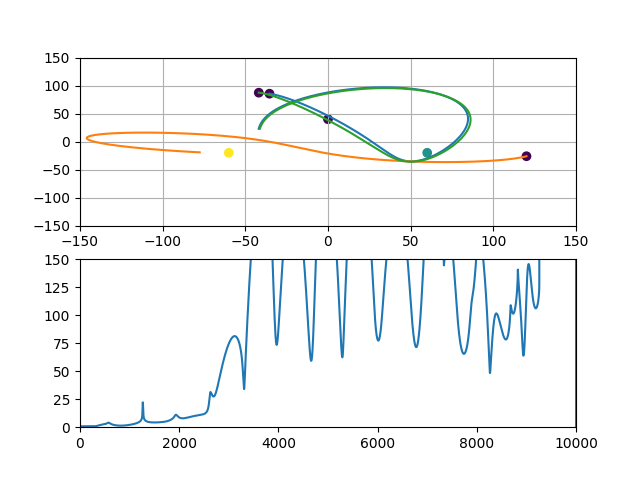
\includegraphics[width=\textwidth]{lyapunov}
\end{frame}

\begin{frame}{Wykładniki Lyapunowa - praktyka}
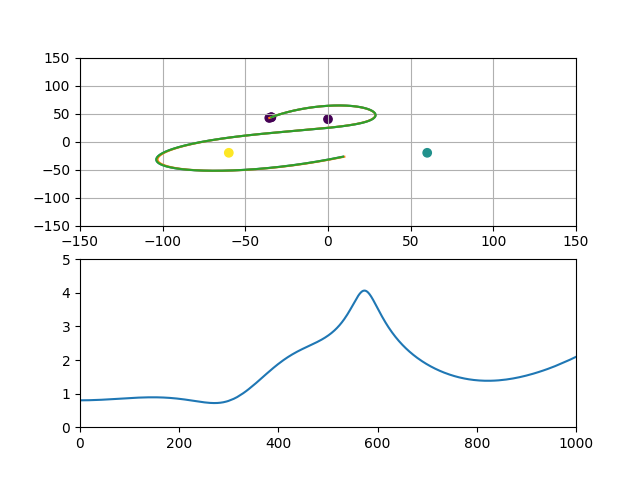
\includegraphics[width=\textwidth]{lyapunov_short}
\end{frame}

\begin{frame}{Wykładniki Lyapunowa - praktyka}
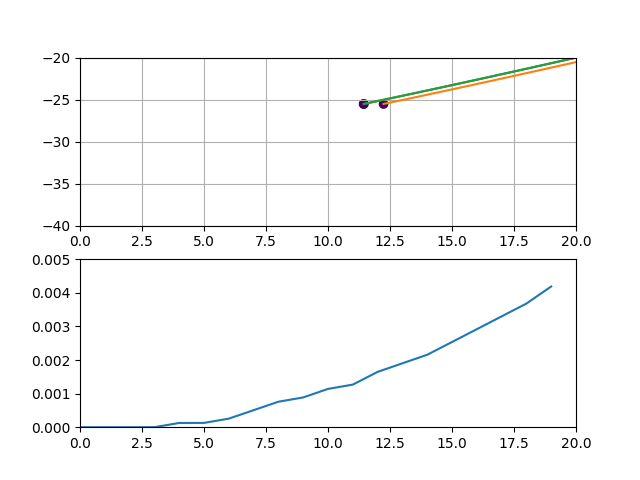
\includegraphics[width=\textwidth]{lyapunov_very_short}
\end{frame}

\begin{frame}
\nocite{stewart1994czy}
\bibliography{mybib}{}
\bibliographystyle{plain}
\end{frame}
\end{document}
